\documentclass{beamer}

\usetheme{Madrid}
\usepackage{wrapfig}
\usepackage[export]{adjustbox}
\usepackage[utf8]{inputenc}
\usepackage{graphicx} %package to manage images
\usepackage{xcolor}
%Information to be included in the title page:
\title{Densities of $k$ Parent Aliquot Numbers}
\author{Gavin Guinn}
\institute{University of Calgary}
\date{June, 2020}

% What are the goals of this presentation?
%Introduce what my project is this summer
% - Extending the pollack and pomerance existing density result 
% - Tabulating existing data on the aliquot sequences so they can be compared to the extended pol/pom result 
% - Scale up computation of delta k estimates
% - generalize the provables lower bounds


%Nice job!  Just one minor comment - I would have put a slide between 4 and 5 giving a high-level statement of your goals (more numerical evidence, conjectural/and provable theoretical results on densities), and then delve deeper starting with Slide 5, working towards your more precise description of your project on Slide 8.  It's important to give an overview early on so your audience has context.


\makeatletter
\newcommand{\subalign}[1]{%
  \vcenter{%
    \Let@ \restore@math@cr \default@tag
    \baselineskip\fontdimen10 \scriptfont\tw@
    \advance\baselineskip\fontdimen12 \scriptfont\tw@
    \lineskip\thr@@\fontdimen8 \scriptfont\thr@@
    \lineskiplimit\lineskip
    \ialign{\hfil$\m@th\scriptstyle##$&$\m@th\scriptstyle{}##$\hfil\crcr
      #1\crcr
    }%
  }%
}
\makeatother

\newcommand\blfootnote[1]{%
  \begingroup
  \renewcommand\thefootnote{}\footnote{#1}%
  \addtocounter{footnote}{-1}%
  \endgroup
}

\begin{document}

\frame{\titlepage}


\begin{frame}
\frametitle{Aliquot Sequences}

\begin{block}{Sum of Divisors}
For any natural number $n$ the sum of divisors of $n$ is defined
$\sigma(n) = \sum_{d|n} d$
\end{block}

And its close relative the sum of proper divisor function
\begin{block}{Sum of Proper Divisors}
$s(n) = \sigma(n) - n$
\end{block}
If $s(m) = n$ then $m$ is known as the parent of $n$ and $n$ is referred to as \textit{aliquot}. It is possible that $n$ could have multiple parents.  \linebreak \linebreak
A number not in the image of $s(\cdot)$ is known as \textit{non-aliquot} or more colourfully as an \textit{aliquot orphan}
\end{frame}

\begin{frame}
\frametitle{Aliquot Sequences, cont}
An aliquot sequence is the iteration of $s(n)$
\begin{align*}
    s(10) &= 1 + 2 + 5\\  
    s(8) &= 1 + 2 + 4\\
    s(7) &= 1\\
    s(1) &= 0
\end{align*}

Above is an example of a sequence terminating after hitting a prime. Sequences can also enter a cycle on a perfect number or on a set of sociable numbers:
$$s(1184) \to s(1210) \to s(1184) \to ...$$
It is an open question whether all aliquot sequences converge or terminate
\begin{block}{Guy-Selfridge Conjecture}
    An infinite amount of aliquot sequences are unbounded 
\end{block}
\end{frame}

\begin{frame}
\frametitle{Natural Density}
For some sequence $S$ of positive integers define a counting function $A(x) = |\{n \in S : 1 \leq n \leq x\}|$ 
\begin{block}{Natural Density of Sequence $S$}
$$d(S)=\lim_{x\to\infty} \frac{A(x)}{x}$$
\end{block}
Natural density is a tool suited for measuring what proportion of all integers belong to the sequence being investigated
\end{frame}

\begin{frame}{Motivation from Dr.Guy}

\small{Think of a number!! Say 36\%, which is nice and divisible. It appears that about 36\% of the even numbers are "orphans". \linebreak

Divide by 1. For about 36\% of the (even) values of n there is just one positive integer m such that s(m) = n. These values of n have just one "parent". \linebreak

Divide by 2.  About 18\% of the even values of n have exactly two parents. \linebreak

Divide by 3. About 6\% of the even values of n have three parents. \linebreak

Divide by 4. About 1 1/2 \% of the even values of n have just 4 parents.  \linebreak

This suggests that 1/(p! e) of the even numbers have p parents.\linebreak

Experiments suggests that these values are a bit large for small values of p and a bit small for larger values of p. Can anything be proved?\\}
\end{frame}

\begin{frame}{Questions}

There already exists an excellent body of work on the density of aliquot orphans, however there seems to minimal work on the densities of $k$ parent aliquot numbers.  \linebreak \linebreak
Let $\Delta_k$ be the natural density of $k$ parent aliquot numbers.\linebreak \linebreak
Dr. Guy's observations raise a couple of questions about $\Delta_k$:
\begin{itemize}
    \item What is the relationship between the calculation of the density of non-aliquots and $\Delta_k$
    \item How do the counts of $k$ parent aliquot numbers compare to density estimates
    \item What has been proved about the similar densities and how can we extend that to $\Delta_k$
\end{itemize}
\end{frame}

\begin{frame}{Existing Work}
    There are two general approaches to the density of non-aliquots:\linebreak\linebreak
    \textbf{Heuristic:}\linebreak
    Pollack and Pomerance (2016) propose a statistical model for the density of non-aliquot numbers. $$\Delta = \lim_{y \to \infty}\frac{1}{\log y} \sum_{\substack{a\leq y \\ 2 | a}} \frac{1}{a}\text{e}^{-a/s(a)}$$
    This approach appears to be highly accurate with $\Delta \approx 0.171822$ and counts of non-aliquot numbers up to $10^{10}$ producing a density of $0.1682$
\end{frame}

\begin{frame}{Existing Work, cont.}
    \textbf{Provable:} \linebreak
    Several authors have produced provable lower bounds for the density of non-aliquot numbers. The most accurate of these would be the work of Chen and Zhao (2011) in which they prove that the set of non-aliquot numbers must make up a set with density greater than \underline{$0.06$}. \linebreak
    
    With the measured density $\approx 0.17$ there seems to be a marked difference between what has been proven and the real density of non-aliquot numbers.
\end{frame}

\begin{frame}{My Project}
    \underline{Goals for this project:} \begin{itemize}
        \item Extend the Pollack and Pomerance probabilistic model for the density of non-aliquot numbers to model $\Delta_k$
        \begin{itemize}
            \item Tabulate counts of $k$ parent aliquot numbers from existing data and compare results to model 
        \end{itemize}
        \item Scale up computation to improve estimates for $\Delta_k$ 
        \item Extend the provable densities of non-aliquot numbers to $k$ parent aliquot numbers
        \begin{itemize}
            \item The plan of attack will be to first extend the lower bound proved by Banks and Luca (2005). The Chen and Zhao paper is not accessible directly through the library. 
        \end{itemize}
    \end{itemize}
\end{frame}

\begin{frame}{Results so Far}
     \begin{block}{Conjectural Density of Aliquot Numbers with $k$ Parents}
    
    $$\Delta_k = \lim_{y \to \infty} \frac{1}{\log y}\sum_{a \leq y} \frac{a^{k-1}}{k! \cdot s(a)^k} \cdot \text{e}^{-a/s(a)}$$
    However there is still work needed to completely justify this result. 
    \end{block}
    
\end{frame}

\begin{frame}{Tentative Numerical Results}
    \begin{center}
{ \small
\begin{table}[]
    \centering
    \begin{tabular}{| c | c | c | c | c | c |}
\hline
 $y$ & $\Delta_0$ & $\Delta_1$ & $\Delta_2$ & $\Delta_3$ & $\Delta_4$ \\ 
 \hline

 50000 & 0.16367 & 0.16577 & 0.09741 & 0.04376 & 0.01651\\
100000 & 0.16458 & 0.16592 & 0.09714 & 0.04351 & 0.01637\\
150000 & 0.16506 & 0.16601 & 0.09699 & 0.04337 & 0.01630\\
200000 & 0.16538 & 0.16606 & 0.09689 & 0.04328 & 0.01625\\
250000 & 0.16561 & 0.16611 & 0.09682 & 0.04321 & 0.01622\\
300000 & 0.16580 & 0.16614 & 0.09676 & 0.04316 & 0.01619\\
\hline
\hline
\hline
 $1/(p! \cdot \text{e})$ & $1/(0! \cdot \text{e})$ & $1/(1! \cdot \text{e})$ & $1/(2! \cdot \text{e})$ & $1/(3! \cdot \text{e})$ & $1/(4! \cdot \text{e})$\\
 \hline
  - & 0.36787 & 0.36787 & 0.18393 & 0.06131 & 0.01532\\
 \hline
 \hline
  $1/2(p! \cdot \text{e})$ & $1/2(0! \cdot \text{e})$ & $1/2(1! \cdot \text{e})$ & $1/2(2! \cdot \text{e})$ & $1/2(3! \cdot \text{e})$ & $1/2(4! \cdot \text{e})$\\
 \hline
  - & 0.18393 & 0.18393 & 0.09196 & 0.03065 & 0.00766\\
  \hline

\end{tabular}
    \caption{Approximation of $\Delta_k$ (restricted to even $a$) compared to Dr. Guy's estimates}
    \label{tab:my_label}
\end{table}

}
\end{center}
{ \small
Where $\frac{1}{p! \cdot e}$ is the estimated density of $k$ parents aliquot numbers over the evens.\\ 
Where $\frac{1}{2(p! \cdot e)}$ is the estimated density of \textbf{even} $k$ parent aliquot numbers over all integers.}
\end{frame}

\begin{frame}{Bounty Problem}
\begin{columns}
\begin{column}{0.5\textwidth}{\small
  Pollack and Pomerance observe that:
   $$|T_a(x)|  \sim  \frac{\phi(A_y) \cdot x}{ A_y \cdot a}$$
    Where:
    \begin{itemize}
    \item $\phi(x)$ is Euler's totient function 
    \item $A_y = \text{ lcm}[1, 2, ..., y]$
    \item $T_a = \{n : \text{gcd}(n, A_y) = a\}$
    \item $T_a(x) = T_a \cap [1,x]$
\end{itemize}
If anyone knows why this holds I'll send you a picture of one the rabbits that live in the park near me}
\end{column}
\begin{column}{0.5\textwidth}  %%<--- here
\begin{center}
    \begin{figure}
    
    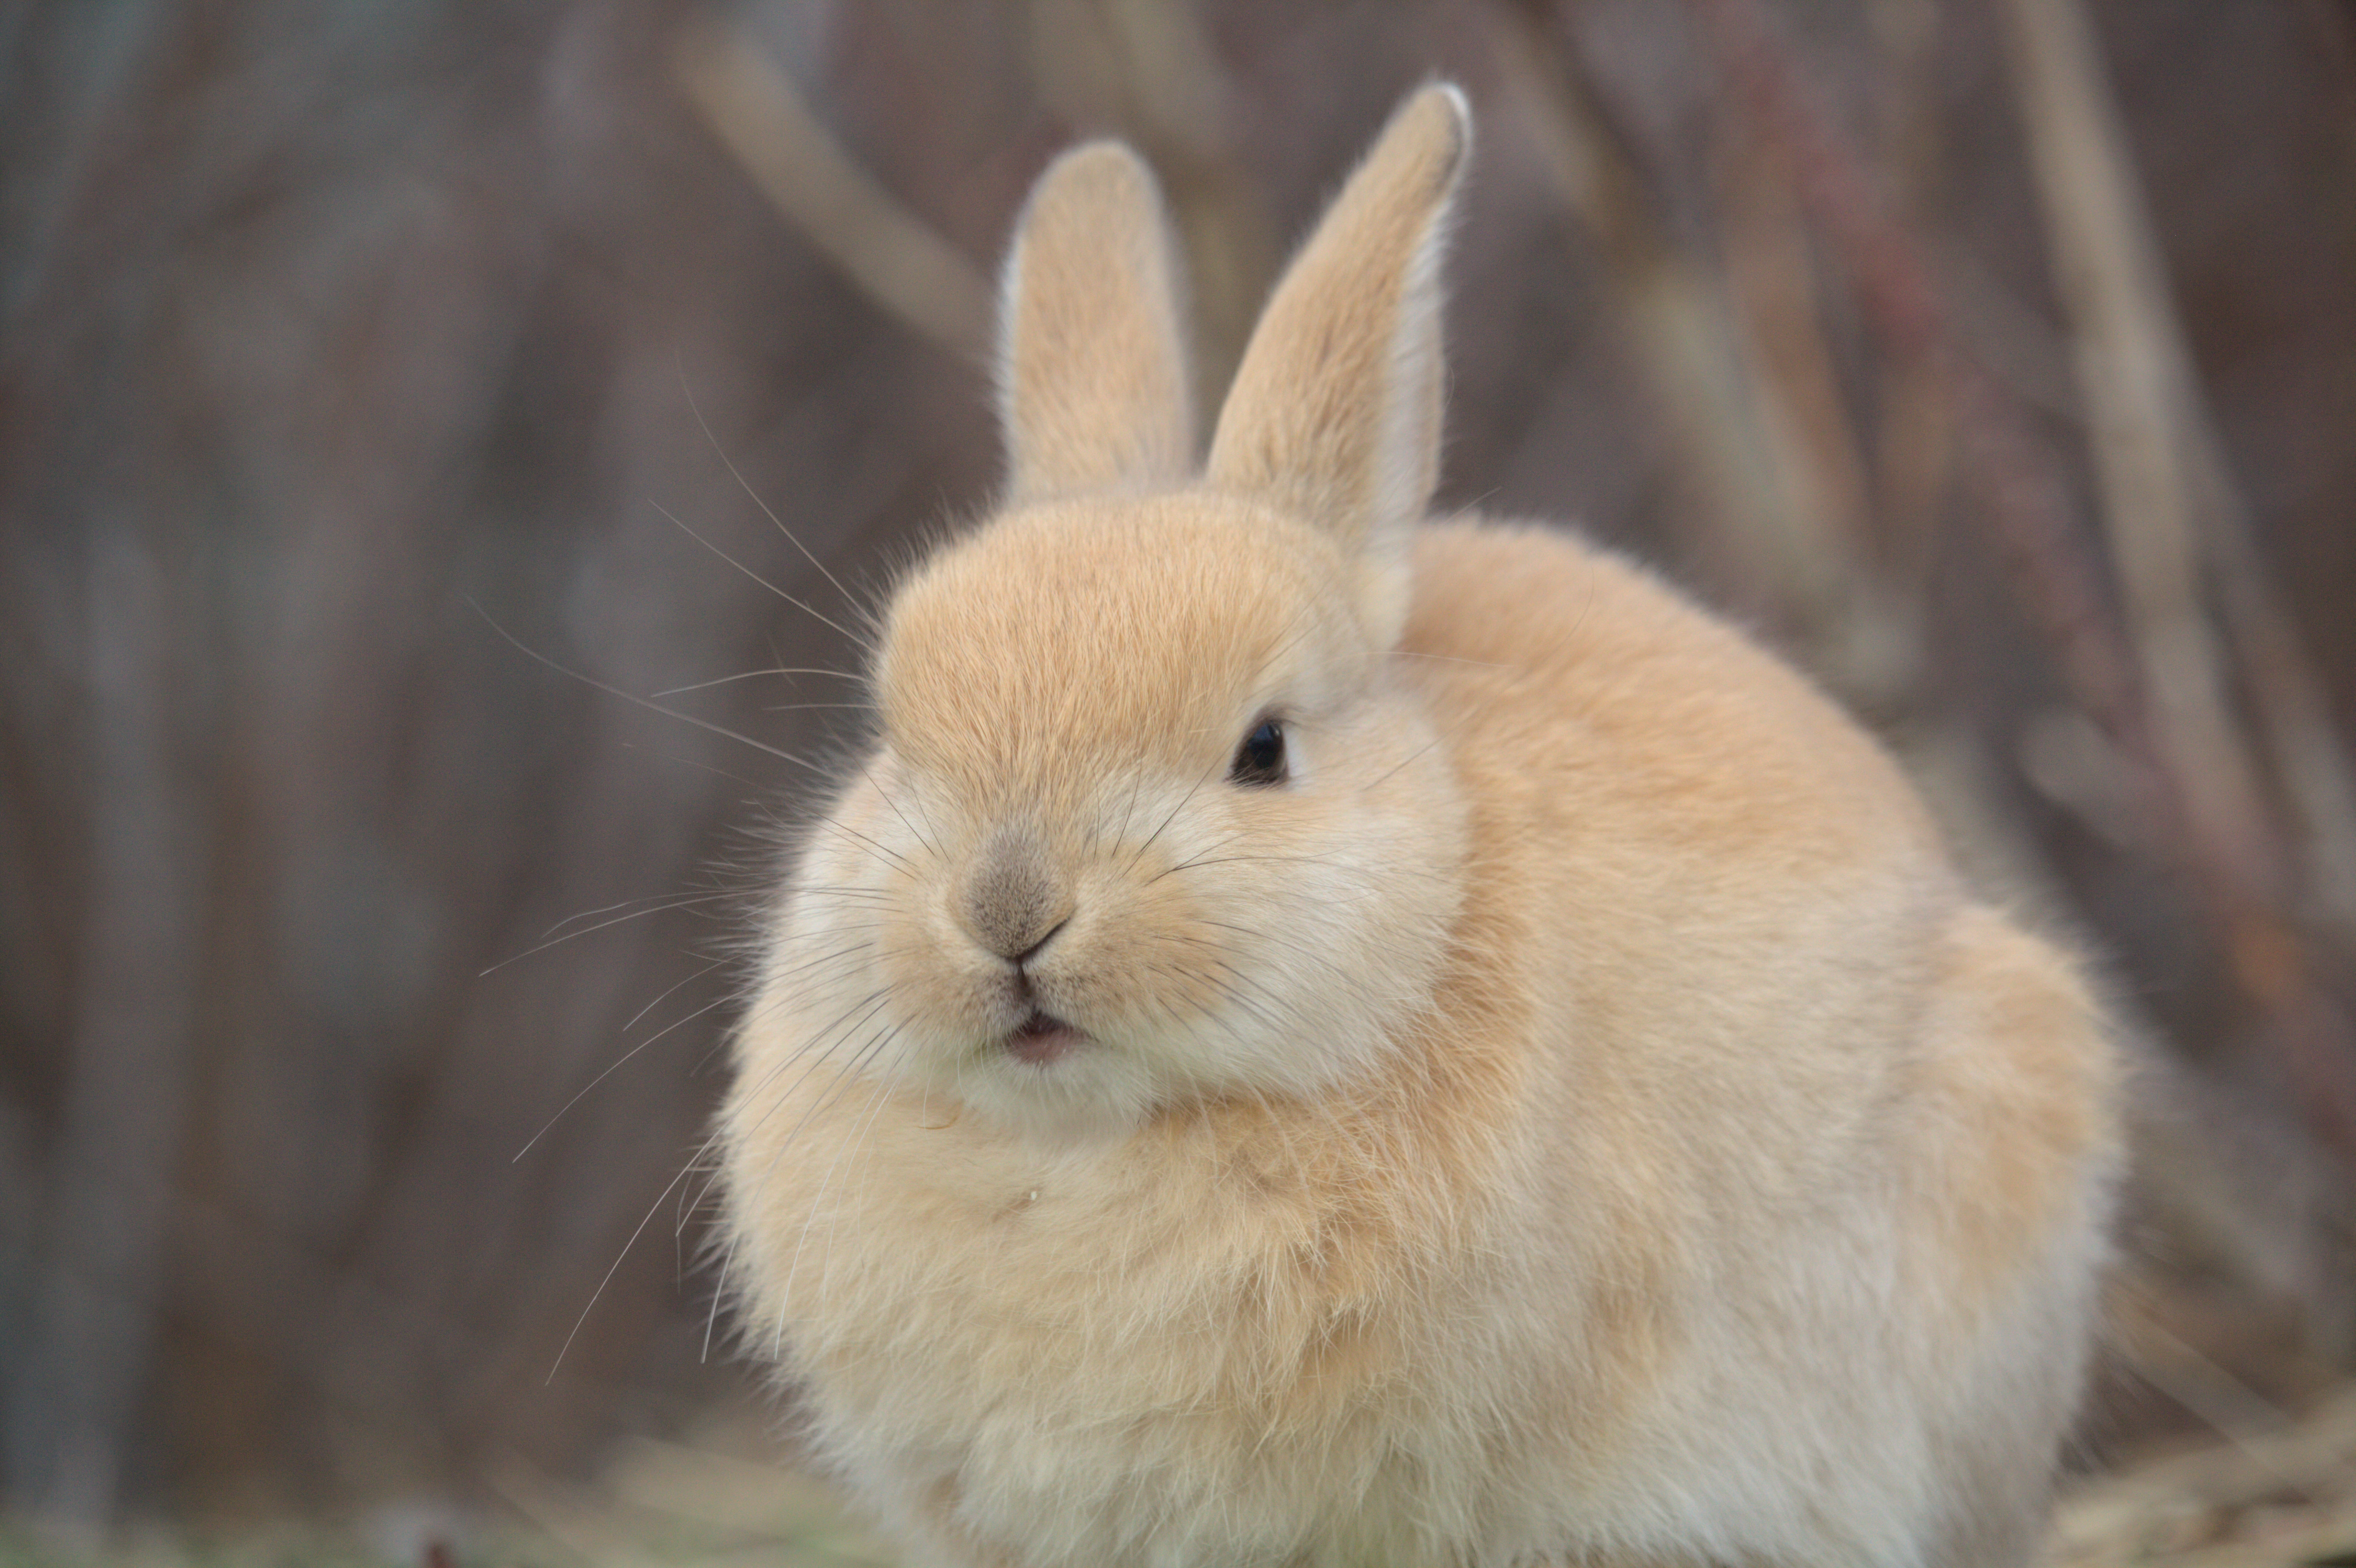
\includegraphics[width=6cm, right]{rabbit.jpg}
    \caption{Example Rabbit}
    \label{fig:my_label}
\end{figure}
\end{center}    
\end{column}
\end{columns}
\end{frame}



\end{document}